\section{Moving objects and Rigid Bodies}
Moving solid objects and rigid bodies are implemented using particles. The only difference between solid objects and rigid bodies is that rigid bodies can rotate and solid objects can not. Objects are defined by a polygon, where the points of the polygon are represented by particles. Forces acting on the particles are directly converted to the object. Furthermore, the center of mass of an object is defined by the location of the object. Lastly, next to the mass of the object, an object has a mass moment of inertia measuring the rigid's ability to resist changes in rotational speed.

\subsection{Boundry conditions}
To make the fluid act more naturally around the boundary of an object, also boundary conditions for objects are introduced. Boundary conditions for objects are defined the same way as boundary conditions for fixed objects. To find the cells of the fluid grid which are on the boundary of the object, we firstly find the bounding box of the object. Then we check for each cell in the bounding box if it contains a part of the boundary of the object or if the cell is completely inside the object.\\
Then for cells which contain a boundary, the same technique as boundary conditions for fixed objects is used. For cells which are inside an object, all components (velocity and density) are set to zero such that they do not have any influence on the object. The downside of setting the fluids density to zero within the object is that the object will remove most of the density, since the boundary force is not sufficient enough to push the fluids away, but it looks more realistic, because the objects leaves a trail as can be seen in figure \ref{fig:trail}.

\begin{figure}[!htb]
\centering
  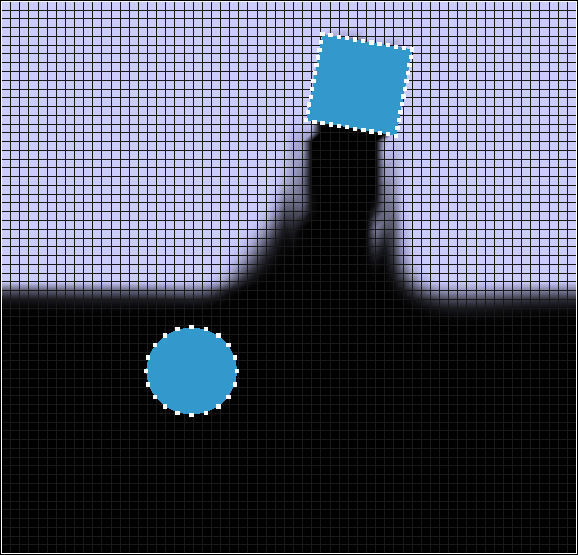
\includegraphics[height=0.5\textwidth]{img/trail}
  \captionof{figure}{Rigid body being dragged by a spring force through the fluid leaving a trail}
  \label{fig:trail}
\end{figure}

\subsection{Object forces}
The total force on an object is defined as $F = \sum{F_i}$, where $F_i$ is the force acting on particle $p_i$ and the total torque on a rigid body is $\tau = \sum{((r_i - x) \times F_i)}$, where $r_i$ is the world position of particle $p_i$. The mass moment of inertia of a body is dependant on the shape of the object. We implemented two type of objects, a rectangle and a disk. The mass moment of inertia $I$ for those object are $I_r =  m (w^2 + h^2)$ and $I_d = \frac{mr^2}{2}$ for a rectangle and a disk respectively.\\
There are two ways in which forces can be applied to an object. Firstly, the fluids pressure can apply forces to the particles of an object as described in the previous section. Secondly the user is able to select one of the particles of an object to create a spring force between the mouse cursor and the particle. Also to make sure an object comes to rest naturally, a drag force is used for both linear and angular velocity. In figure \ref{fig:fluidobject} it can be seen that the fluid exerts force on rigid bodies.
\begin{figure}[!htb]
\centering
  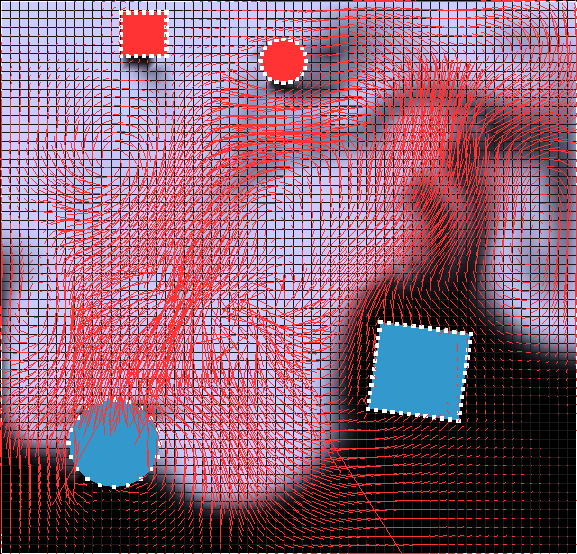
\includegraphics[height=0.5\textwidth]{img/fluidobject}
  \captionof{figure}{Moving solids (red) and rigid bodies (blue) being moved by forces exerted by the fluid}
  \label{fig:fluidobject}
\end{figure}
\subsection{Object to fluid coupling}
To make the simulation more realistic, solid objects and rigid bodies also exert forces to the fluids. This is done by adding velocity to the velocity field around the object. To find the cells around the object, just like with the boundary conditions, we find the bounding box of the object and then find the cells which contain a part of the boundary of the object. Then for the cells next to the boundary, we add a fraction of objects velocity to these cells, such that the density around the object will also be advected in the direction in which the object is moving. The influence of the object on the velocity field can be seen in figure \ref{fig:objectfluid}.

\begin{figure}[!htb]
\centering
  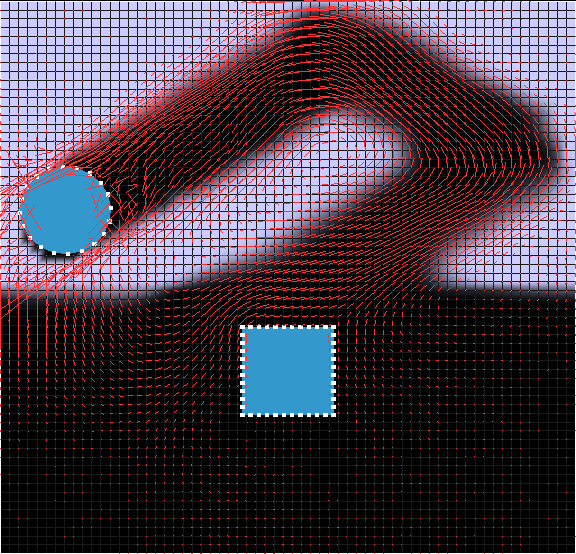
\includegraphics[height=0.5\textwidth]{img/objectfluid}
  \captionof{figure}{Moving rigid body influences velocity field}
  \label{fig:objectfluid}
\end{figure} 